\documentclass[10pt,landscape,a4paper]{article}
\usepackage{multicol}
\usepackage[landscape]{geometry}
\usepackage{hyperref}
\usepackage[utf8]{inputenc}
\usepackage{minted}
\usepackage{graphicx}
\graphicspath{ {./images/} }
\usepackage[binary-units]{siunitx}
\usepackage[x11names]{xcolor}
\usepackage{textcomp}

\geometry{top=1cm,left=1.5cm,right=1cm,bottom=1cm}

\usepackage{tgheros}
\renewcommand{\familydefault}{\sfdefault}


% LAYOUTING MOSTLY 'INSPIRED' BY The-Compiler ( https://github.com/The-Compiler )

% Turn off header and footer
\pagestyle{empty}
 
% Redefine section commands to use less space
\makeatletter
\renewcommand{\section}{\@startsection{section}{1}{0mm}%
                                {-1ex plus -.5ex minus -.2ex}%
                                {0.5ex plus .2ex}%x
                                {\normalfont\large\bfseries}}
\renewcommand{\subsection}{\@startsection{subsection}{2}{0mm}%
                                {-1explus -.5ex minus -.2ex}%
                                {0.5ex plus .2ex}%
                                {\normalfont\small\bfseries}}
\renewcommand{\subsubsection}{\@startsection{subsubsection}{3}{0mm}%
                                {-1ex plus -.5ex minus -.2ex}%
                                {1ex plus .2ex}%
                                {\normalfont\footnotesize\bfseries}}
\renewcommand{\paragraph}{\@startsection{paragraph}{3}{\z@}%
                                {-1ex plus -.5ex minus -.2ex}%
                                {-.5em}%
                                {\normalfont\scriptsize\bfseries}}
\makeatother

% Don't print section numbers
\setcounter{secnumdepth}{0}

\setlength{\parindent}{0pt}
\setlength{\parskip}{0pt plus 0.5ex}

% Compact lists
\usepackage{enumitem}
\setlist{nosep}

% -----------------------------------------------------------------------

\begin{document}

\footnotesize
\begin{multicols*}{4}

% multicol parameters
% These lengths are set only within the two main columns
\setlength{\columnseprule}{0.25pt}
\setlength{\premulticols}{1pt}
\setlength{\postmulticols}{1pt}
\setlength{\multicolsep}{1pt}
\setlength{\columnsep}{2pt}



%OS-STUFF
\section{Various OS-Stuff}

\subsection{Kernellevel}
\begin{description}
  \item[Kernel Mode] Alle Instruktionen
  \item[User Mode] Beschränktes Instruktionsset
\end{description}

Elevate User\textrightarrow~Kernel via \textit{syscall}

Jede Kernelfunktion hat spezifischen Code (e.g. \textit{exit}\textrightarrow~\textit{60}), weitere Args via definierter Register

\subsection{ENV Variables}
\begin{itemize}
    \item OS-Verwaltet
    \item Array von Key=Value Paaren
    \item Stored in \textit{environ}
\end{itemize}
Zugriffe:\\
\mintinline{C}{char* getenv (const char* k)} [not found \textrightarrow~ret 0]\\
\mintinline{C}{int setenv(const char* k, const char* v,}\\
\mintinline{C}{ int o) //o != 0 -> overwrite existing}\\
\mintinline{C}{int unsetenv(const char* k) //remove var}\\
\mintinline{C}{int putenv (char* kvp) //add/replace mit ptr}



%Filesystems
\section{Dateisysteme}
\begin{description}
  \item[Verzeichnis] \textit{directory} \textrightarrow~Datei mit Liste aller Dateien
  \item[Verzeichnishierarchie] Baum-Struktur
  \item[Wurzelverzeichnis] \textit{root directory} \textrightarrow~/
  \item[Kanonische Pfade] Ohne \textit{.} und \textit{..} \textrightarrow~\textit{realpath}
\end{description}

\subsection{Zugriffsrechte}

1 Oktal-Zahl/3 Bit each: \textcolor{Firebrick1}{Owner}, \textcolor{Chartreuse2}{Group}, \textcolor{Goldenrod1}{World}\\
\textbf{r}ead: 4 / 100\textsubscript{b} \textbf{w}rite: 2 / 010\textsubscript{b} e\textbf{x}ecute): 1 / 001\textsubscript{b}\\
\textcolor{Firebrick1}{rwx}\textcolor{Chartreuse2}{r--}\textcolor{Goldenrod1}{---} $\rightarrow$ 0\textcolor{Firebrick1}{7}\textcolor{Chartreuse2}{4}\textcolor{Goldenrod1}{0}



%C
\section{C}
\begin{description}
  \item[Präprozessor] verarbeitete Kommentare \& Makros
  \item[Compiler] Kompiliert C \textrightarrow~Assembly
  \item[Assembler] Übersetzt Assembly zu Objectdatei
  \item[Linker] Löst Referenzen auf
\end{description}

\subsection{Programmargumente}
\mintinline{C}{int main (int argc, char** argv)} [num-args; arg-array-pointer \textrightarrow~\textbackslash0-terminierte Abschnitte]

\subsection{Filesystem API [CHAR DATA]}
\verb|fdopen(fd, char *mode) -> FILE| \\
\verb|fopen(path, mode) -> FILE| \\
\verb|fgets(char *outs, n, stream) -> int| \\
\verb|fputs(int c, stream) -> status| \\
\verb|fseek(stream, offset, whence) -> status| \\
\verb|rewind(stream)|: \verb|fseek(stream, 0, SEEK_SET)|, clear errno



%POSIX
\section{POSIX}

\subsection{Filesystem API [BINARY DATA]}
\begin{description}
  \item[File-Descriptor] \textit{fd} \textrightarrow~nur innerhalb Prozess, Index auf Filedeskriptor-Tabelle, \textit{integer}
  \item[File-Deskriptor-Tabelle] alle geöffneten Dateien vom Prozess, Index auf systemweite Tabelle, Zustandsbehaftet (read-offset)
  \item[Global-Descriptor-Table] enthält Daten um physische Datei zu identifizieren (Treiber, Datenträger, etc.)
\end{description}

\smallskip

\verb|open(path, flags) -> fd|, \\
\verb|close(fd) -> status|, \\
\verb|read/write(fd, buffer, n) -> status [n bytes]|, \\
\verb|pread| und \verb|pwrite| mit Offset als Argument \\
\verb|lseek(fd, offset, whence) -> status|,

\smallskip

\subsection{Thread API}
\begin{minted}{c}
int pthread_create (
pthread_t* thread_id, //Out-Parameter
pthread_attr_t const* attributes,
void* (*start_function) ( void*),
void* argument)
\end{minted}
! \mintinline{C}{argument} sollte auf den HEAP verweisen um nicht ausversehen abgebaut zu werden !
\smallskip
Ein Thread lebt bis eine der folgenden Bedingungen eintritt:\\
\begin{minipage}[t]{\textwidth}
    \begin{itemize}[nosep]
        \item return aus \mintinline{C}{start_function}
        \item ruft \mintinline{C}{pthread_exit(void* rv)} auf
        \item anderer Thread ruft \mintinline{C}{pthread_cancel(id)} auf
        \item parent-Prozess wird beendet
    \end{itemize}
\end{minipage}

\smallskip

\subsection{Messaging API}
\begin{minted}{C}
mqd_t mq_open(const char* name, int flags,
          mode_t mode, struct mq_attr* attr)
int mq_close(mqd_t queue)
//mark for kill when not used anymore
int mq_unlink(const char* name)
int mq_send(mqd_t queue, const char* msg,
       size_t length, unsigned int priority)
int mq_receive(mqd_t queue, const char* msg,
      size_t length, unsigned int* priority)
\end{minted}



%Prozesse
\section{Prozesse}
\begin{description}
  \item[Monoprogrammierung] Nur 1 Prozess \& Betriebssystem auf Prozessor
  \item[Quasi-Parallel] Mehrere Prozesse auf Prozessor, Scheduling um Ressourcen zu verteilen
  \item[Process Control Block] \textit{PCB} Speicher für alle Daten die OS benötigt um Prozess ins System zu integrieren (ID, Parent-ID, Speicher, Scheduling-Infos, Messaging, FS-handles, Security
  \item[PCB Kontext-Save] Register, Flags, Instruction Pointer, MMU-Konfig (Page-Table-Pointer)
\end{description}

\smallskip

\begin{description}
  \item[Interrupt] Kontext wird gesichert, Interrupt-Handler aufrufen (kann Kontext modifizieren), Kontext wiederherstellen
  \item[Kontextwechsel] Wechsel von Prozess \textit{X} auf Prozess \textit{Y}. Kontext A wird gesichert, Kontext B wird wiederhergestellt
\end{description}

\subsection{Forking, Zombies, Verwaisung}
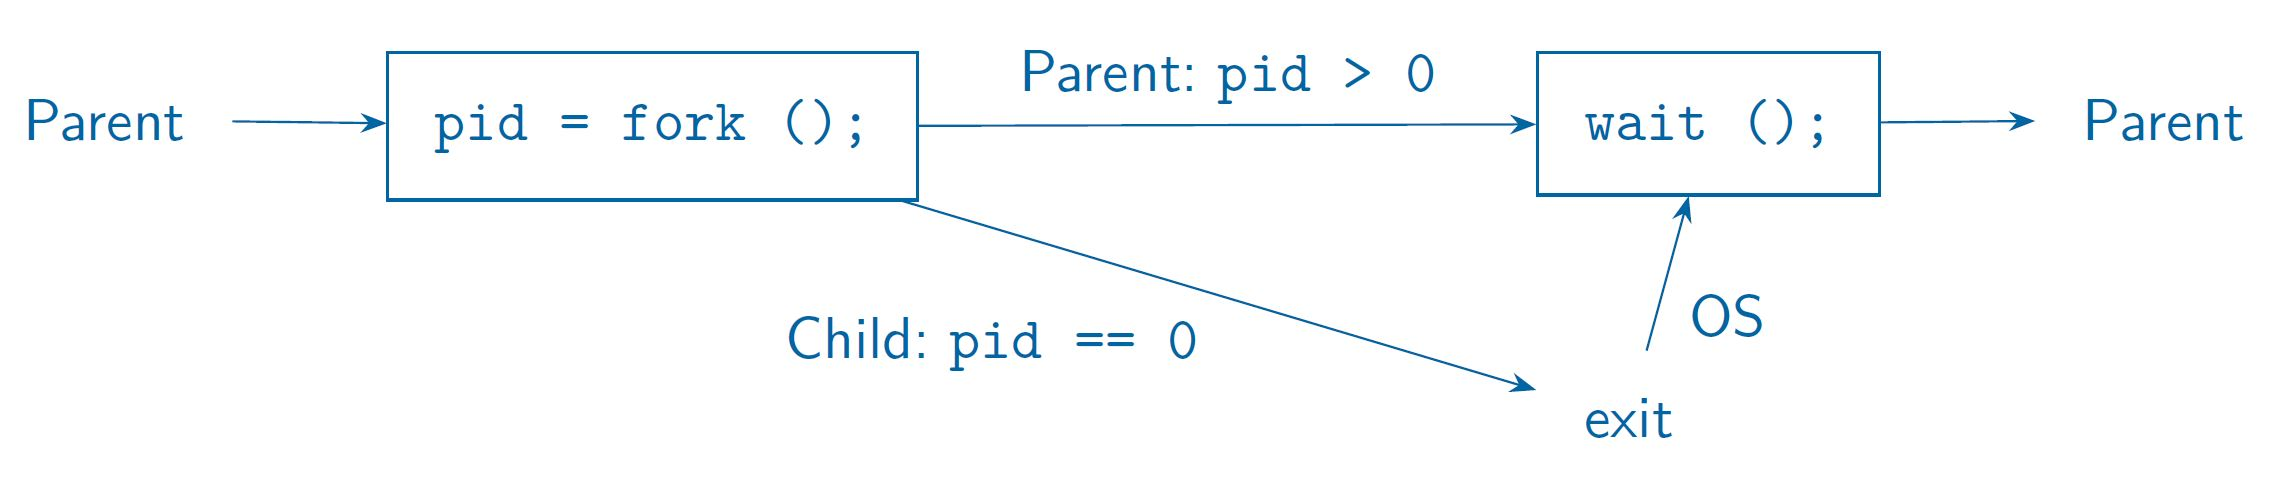
\includegraphics[width=1.0\linewidth]{01_forking.JPG}
\begin{description}
  \item[Zombieprozess] Childprozesse können vom OS erst entfernt werden wenn Parent \mintinline{C}{wait()} aufruft \textrightarrow~Child ist bis dann ein \textit{Zombie}
  \item[Orphanprozess] Wird Parentprozess beendet bevor Child fertig ist, hat Child keinen Parent mehr \textrightarrow~\textit{verwaist} und kann nicht beendet werden \textrightarrow Beim Beenden eines Prozesses werden darum alle Childprozesse an den \textit{kill-Prozess} [pid = 1] übertragen, dieser ruft kosntant \mintinline{C}{wait()} auf um Childprozesse zu töten
\end{description}



%Threads
\section{Threads}
\begin{description}
  \item[Thread Control Block] \textit{TCB} kongruent zu Prozessen braucht ein Thread einen eigenen Stack, etc. Unter Linux hat jeder Thread eine Kopie des PCB \underline{aber mit eigenem Kontext}
\end{description}

\subsection{Amdahls Regel}
\begin{description}
    \item[$\textcolor{Chartreuse1}{n}$]n-Prozessoren
    \item[$\textcolor{Firebrick1}{T}$]Ausführungszeit, wenn komplett seriell ausgeführt
    \item[$T'$]Zeit, wenn max. parallelisiert ($\textcolor{brown}{\textcolor{brown}{T_{s}}} + \frac{\textcolor{Firebrick1}{T}-\textcolor{brown}{\textcolor{brown}{\textcolor{brown}{T_{s}}}}}{\textcolor{green}{n}}$)
    \item[$\textcolor{brown}{\textcolor{brown}{\textcolor{brown}{T_{s}}}}$]Zeit, serieller Anteil
    \item[$\textcolor{Firebrick1}{T} - \textcolor{brown}{\textcolor{brown}{\textcolor{brown}{T_{s}}}}$]Zeit, parallelisierbarer Anteil
    \item[$\frac{\textcolor{Firebrick1}{T} - \textcolor{brown}{\textcolor{brown}{\textcolor{brown}{T_{s}}}}}{\textcolor{green}{n}}$]Parallel-Anteil verteilt auf n-Prozessoren
    \item[$\textcolor{blue}{s} = \frac{\textcolor{brown}{T_s}}{\textcolor{Firebrick1}{T}}$]serieller Anteil Algorithmus
\end{description}

\subsubsection{Speedup-Faktor}
$f \le \frac{\textcolor{Firebrick1}{T}}{T'} = \frac{\textcolor{Firebrick1}{T}}{\textcolor{brown}{\textcolor{brown}{\textcolor{brown}{T_{s}}}} + \frac{\textcolor{Firebrick1}{T} - \textcolor{brown}{\textcolor{brown}{\textcolor{brown}{T_{s}}}}}{\textcolor{green}{n}}} = \frac{\textcolor{Firebrick1}{T}}{\textcolor{blue}{s} \cdot \textcolor{Firebrick1}{T} + \frac{\textcolor{Firebrick1}{T}-\textcolor{blue}{s}\cdot \textcolor{Firebrick1}{T}}{\textcolor{green}{n}}} = \frac{\textcolor{Firebrick1}{T}}{\textcolor{blue}{s} \cdot \textcolor{Firebrick1}{T} + \frac{1-\textcolor{blue}{s}}{\textcolor{green}{n}} \cdot \textcolor{Firebrick1}{T}} = \frac{1}{\textcolor{blue}{s} + \frac{1-\textcolor{blue}{s}}{\textcolor{green}{n}}}$\\
parallele Variante ist maximal $f$-mal schneller

\subsubsection{Bedeutung}
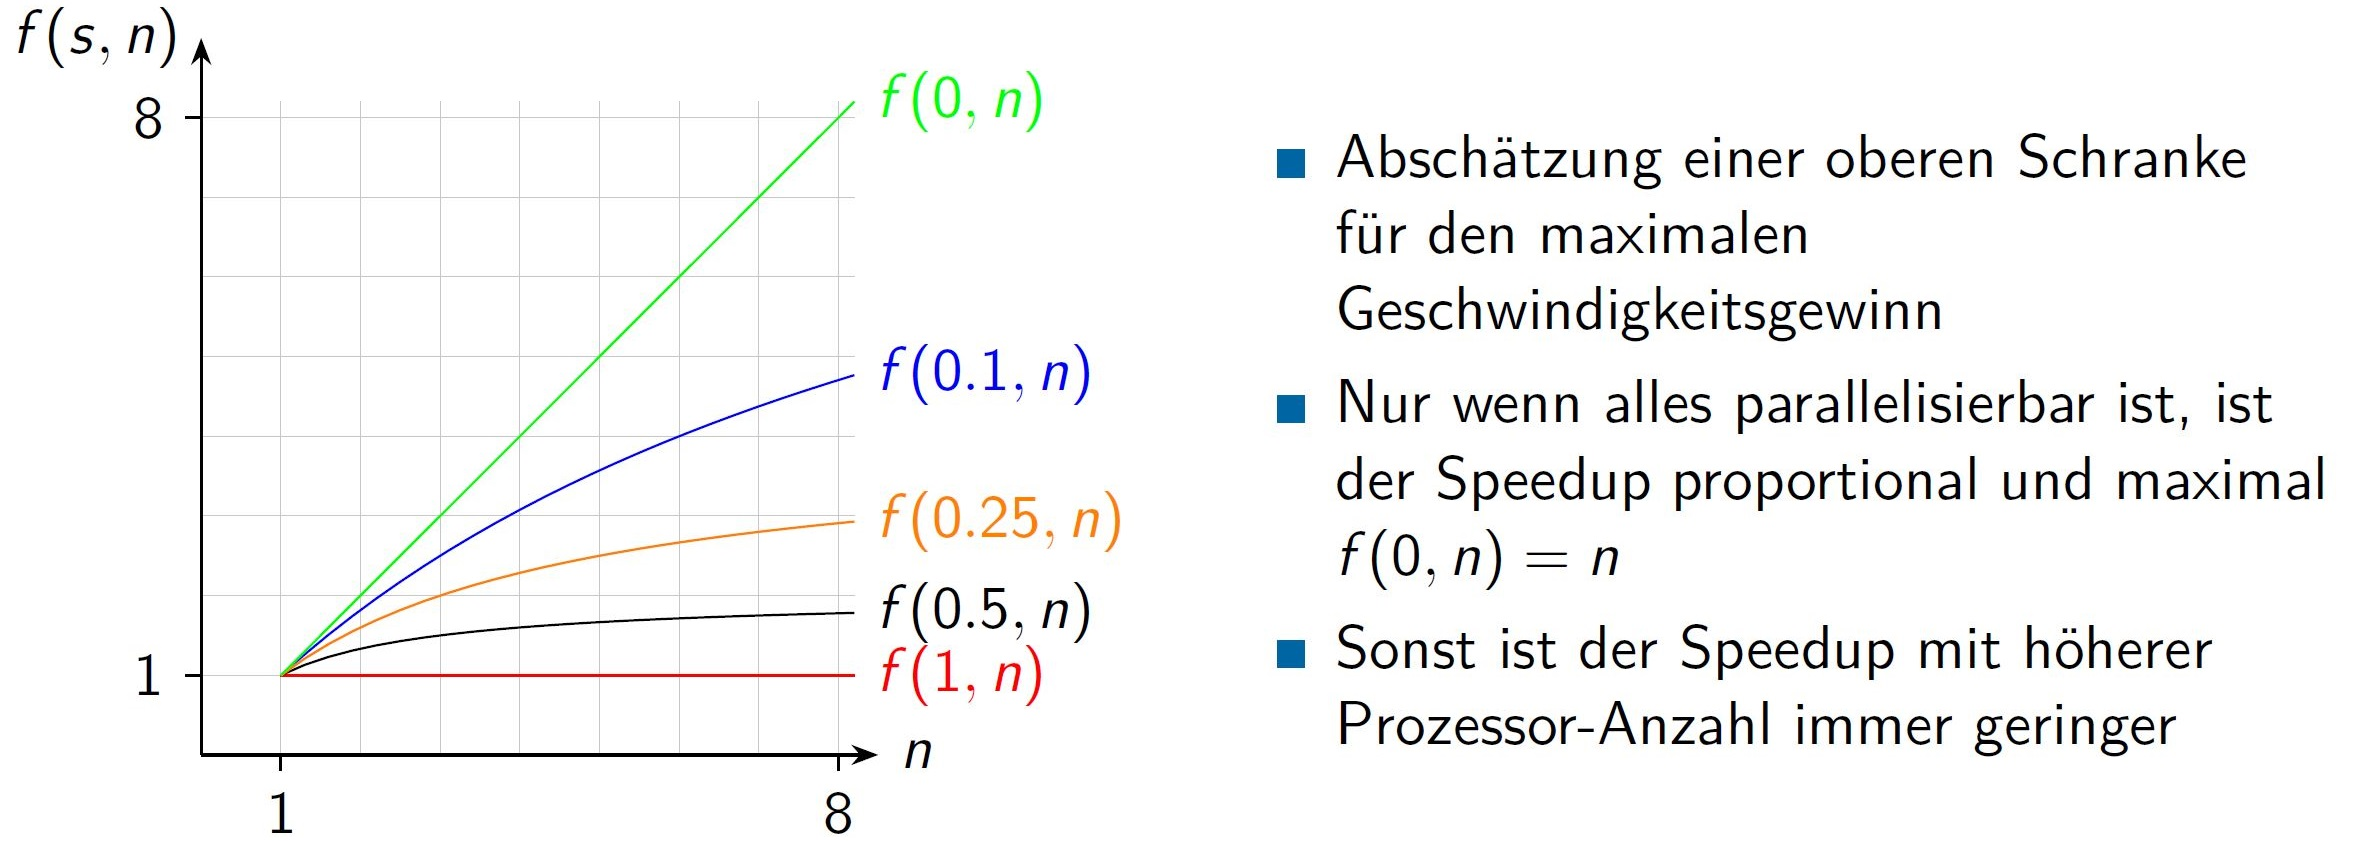
\includegraphics[width=1.0\linewidth]{02_amdahl_graph.JPG}

\subsection{Scheduling}
\begin{description}
  \item[Zustände] in denen sich ein Thread befinden kann:
  \begin{description}
    \item[running] aka \textit{Prozessor-Burst}, Thread is aktiv
    \item[ready] alle Threads die aktiv sein könnten
    \item[waiting] aka \textit{I/O-Burst}, wartet auf Externes Ereignis (e.g. Input)
  \end{description}
  \item[Übergänge] werden vom OS durchgeführt
  \item[Ready-Queue] Datenstruktur (bspw Tree) in der \textit{ready} Threads warten
  \item[Standby] der Prozessor schaltet in einen Energiespaarmodus wenn alle Threads warten
  \item[Kooperativ] Thread entscheidet wann er dem Prozessor erlaubt zu Schedulen (\textit{yield})
  \item[Präemptiv] Scheduler entscheidet wann ein Thread pausieren muss
  \item[Parallel] \textit{n} Threads benötigen \textit{n} Prozessoren
  \item[Quasiparallel] \textit{n} Threads auf \textit{\textless n} Procs aufgeteilt
  \item[Scope] Die meisten OS' laufen in System-Contention
  \begin{description}
    \item[Process-Contention Scope] Scheduling nur innerhalb des aktiven Threads
    \item[System-Contention Scope] Scheduling über das gesamte System
  \end{description}
\end{description}

\smallskip

Anforderungen an Scheduler (nicht alle möglich):
\begin{description}
  \item[Closed-System] kann perfekt optimiert werden (e.g. Embedded)
  \item[Open-System] e.g. OS, wird an grössten Verwender angepasst
  \item[turnaround time] möglichst kurze Threadlebenszeit
  \item[response time] schnelle Reaktion auf requests
  \item[waiting time] threads sollen möglichst wenig warten
  \item[throughput] anzahl Threads die per Interval bearbeitet werden
  \item[processor utilization] aktive Prozessor Verwendung vs waiting
  \item[latency] Zeit zwischen Auftreten und Verarbeitung eines Ereignisses
\end{description}

\subsubsection{Mögliche anstehende Threads}
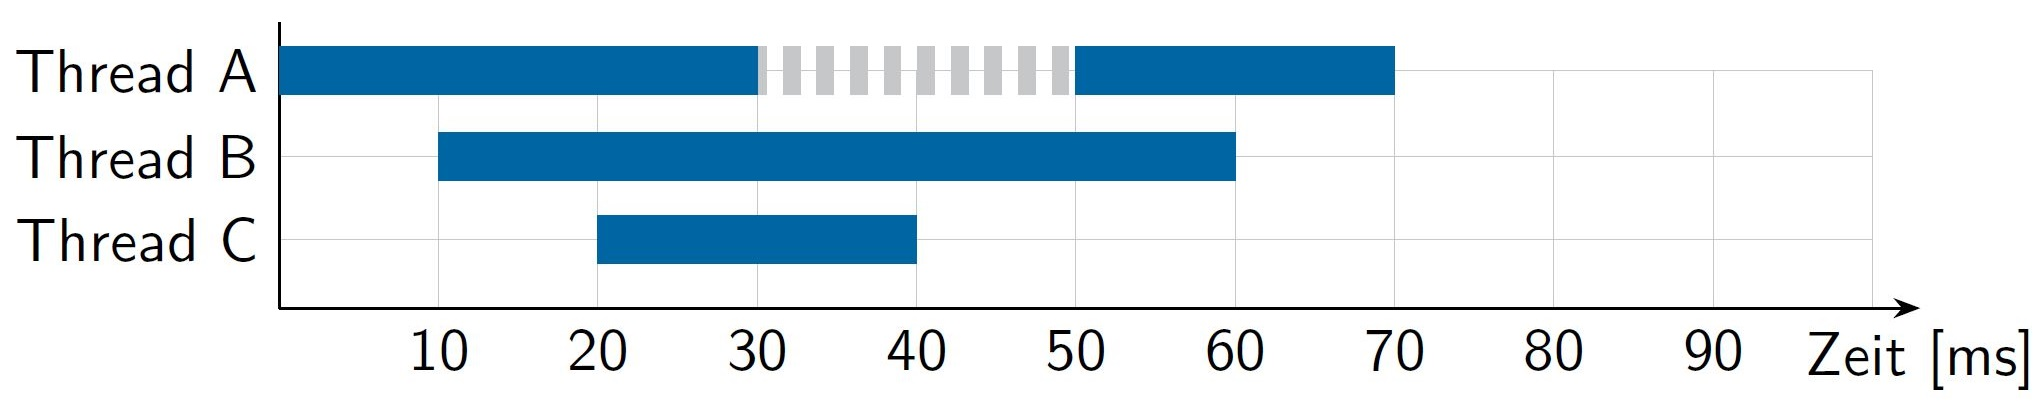
\includegraphics[width=1.0\linewidth]{03A_scheduling_base.JPG}

\includegraphics[width=1.0\linewidth]{03_legende.JPG}

\subsubsection{FCFS (FIFO-Geordnet, mögl. \textcolor{RoyalBlue4}{Priorisierung}}
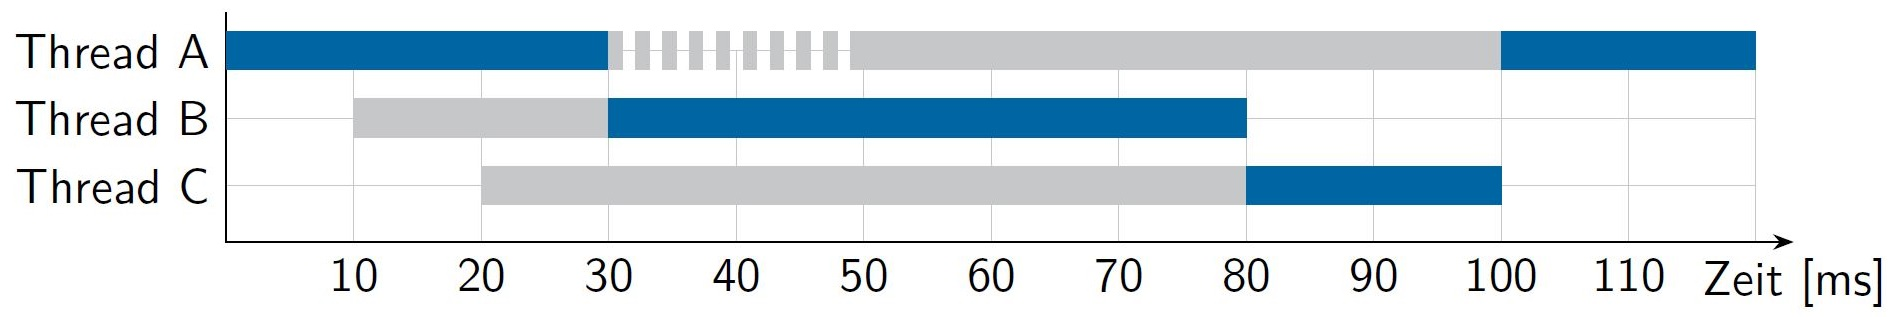
\includegraphics[width=1.0\linewidth]{03B_FCFS.JPG}

\subsubsection{SJF (Shortest Job First; \textcolor{RoyalBlue4}{Koop} oder Prä)}
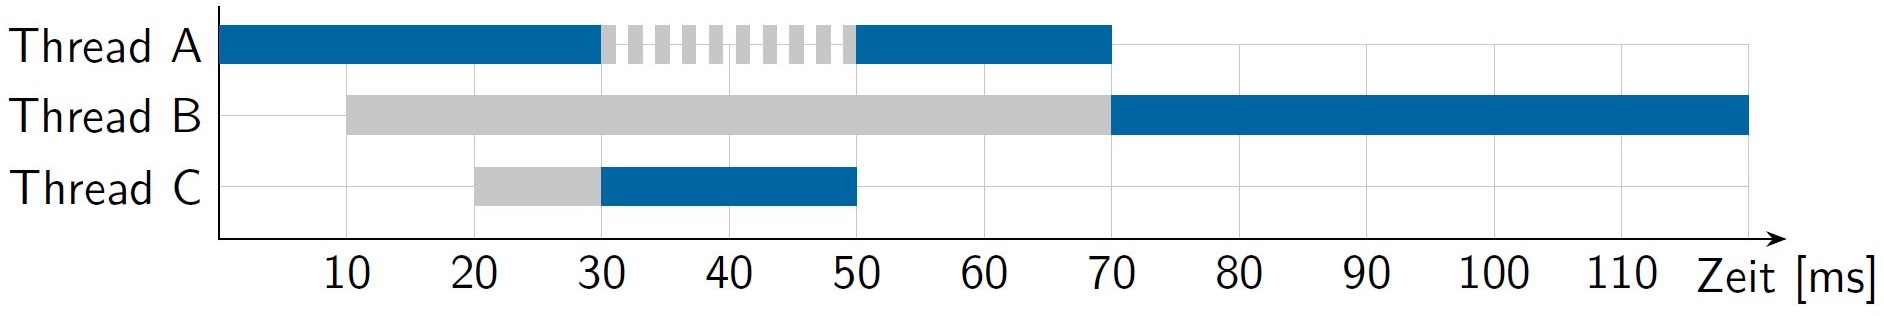
\includegraphics[width=1.0\linewidth]{03C_SJF.JPG}

\subsubsection{Round-Robin (Time Sliced \textcolor{RoyalBlue4}{10}-100ms)}
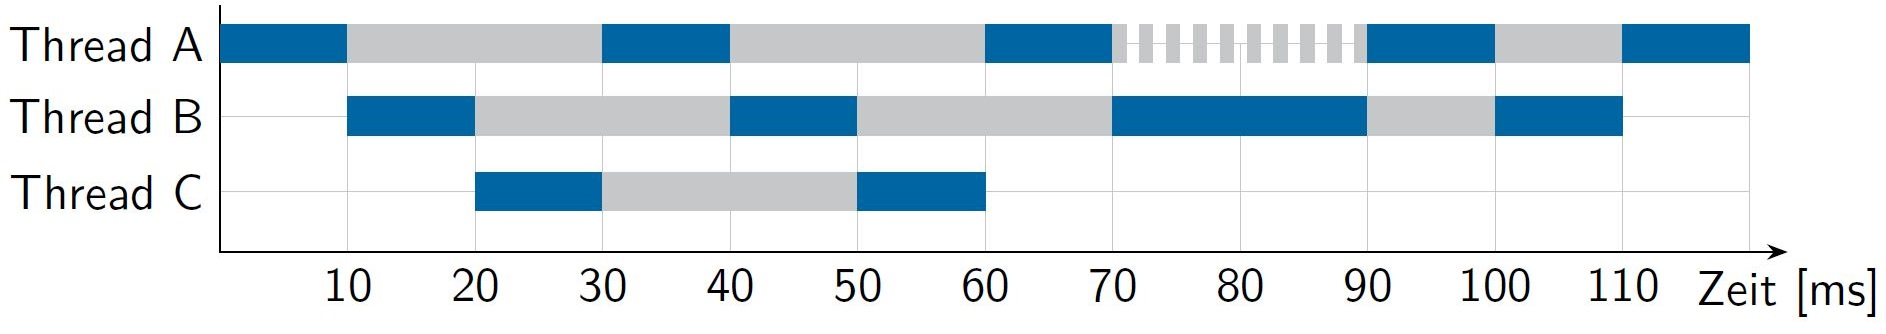
\includegraphics[width=1.0\linewidth]{03D_RR.JPG}



%Synchronization, Mutex, Semaphore, etc.
\subsection{Synchronisation}
\begin{description}
  \item[Critical Section] Codebereich eines Threads in welchem er Daten mit anderen Threads teilt
  \item[Abschalten von Interrupts] unpraktisch \& gefährlich, OS kann Thread nicht mehr unterbrechen
  \item[Semaphor] Zähler \mintinline{C}{z}, \mintinline{C}{post}-funktion inkrementiert, \mintinline{C}{wait}-funktion dekrementiert, wenn \mintinline{C}{z == 0} warten bis anderer thread \mintinline{C}{post}et
  \item[Mutex] aka \textit{lock}, \mintinline{C}{acquire} setzt lock auf 1 und blockiert weitere \mintinline{C}{acquire}-calls, \mintinline{C}{release} setzt lock auf 0
\end{description}



%Messaging und Co
\section{Kommunikation}

\subsection{Signale}
\begin{description}
  \item[Fancy Interrupts] Signale können auch von anderen Prozessen gesendet werden
  \item[Signal Handler] wird beim Prozessstart gesetzt, kann vom Programm überschrieben werden
\end{description}
\begin{minted}{C}
int sigaction(int sig, struct sigaction *new,
              struct sigaction *old)
\end{minted}

\subsubsection{Programmfehler}
\begin{description}
  \item[SIGFPE] Floating Point Error
  \item[SIGILL] Ungültige Instruktion
  \item[SIGSEGV] Ungültiger Speicherzugriff
  \item[SIGSYS] Ungültiger Systemaufruf
\end{description}

\subsubsection{Prozesse Abbrechen}
\begin{description}
  \item[SIGTERM] \textit{höfliche} Anfrage
  \item[SIGINT] aka \textit{Ctrl + C} \textrightarrow~Cancel
  \item[SIGQUIT] aka \textit{Ctrl + \textbackslash} \textrightarrow~Abort
  \item[SIGABRT] Abort, aber vom Prozess an sich selbst
  \item[SIGKILL] Terminate, \underline{nicht überschreibbar}
\end{description}

\subsubsection{Stop \& Continue}
\begin{description}
  \item[SIGTSTP] aka \textit{Ctrl + Z} \textrightarrow~Stop / background
  \item[SIGSTOP] Stop, aber \underline{nicht überschreibbar}
  \item[SIGCONT] aka \textit{fg} \textrightarrow~foreground
\end{description}

\subsection{Pipes}
\begin{description}
  \item[Fake Datei] erzeugt POSIX \textit{fd}s für Ein- und Ausgang
  \item[Interprozesskommunikation] auf Systemebene
  \item[Size] default 16 Pages (4KB-pages \textrightarrow~64KB)
\end{description}
\mintinline{C}{int pipe(int fd [2])}

\subsection{Sockets}
\begin{description}
  \item[Intersystemkommunikation] so mit LAN \& Internet
  \item[Eindeutiger Name] wird benötigt um fremden Socket zu finden (bsp \textcolor{DarkOliveGreen2}{IP}:\textcolor{DarkOrange2}{Port})
\end{description}
\mintinline{C}{int socket(int domain, int type, int prot)}
\mintinline{C}{int bind(...)}, \mintinline{C}{int connect(...)},\\
\mintinline{C}{int listen(...)} \& \mintinline{C}{int accept(...)}

\subsection{Message-Passing}
\begin{description}
  \item[Send] kopiert Nachricht \textit{aus} dem Prozess
  \item[Receive] kopiert Nachricht \textit{in} den Prozess
  \item[Direkt] Sender muss Empfänger kennen
  \begin{description}
    \item[Symmetrisch] Empf. muss Sender kennen
    \item[Assymetrisch] Empfänger erhält eine \textit{msg-id} beim Abfragen neuer Nachrichten
  \end{description}
  \item[Indirekt] funktioniert via Datenstruktur die beide kennen (e.g. Message-Queue)
  \item[Rendevouz] Sender \& Empfänger blockieren
\end{description}

\subsection{Shared Memory}
\begin{description}
  \item[Selbes Frame] wird für mehrere Prozesse benutzt
  \item[Synchronisierung] nötig (e.g. via Mutex)
  \item[Pointer] müssen relativ zu einer Anfangsaddr sein
\end{description}



%X-Window...
\section{X-System}
\begin{description}
  \item[Universell] Teil von Linux, definiertes Protokoll
  \item[Display] Usersystem (e.g. thinclient wie Sun Ray)
  \item[X Server] Software die Displays ansteuert
  \item[X Client] Applikation die Display nutzen will
\end{description}
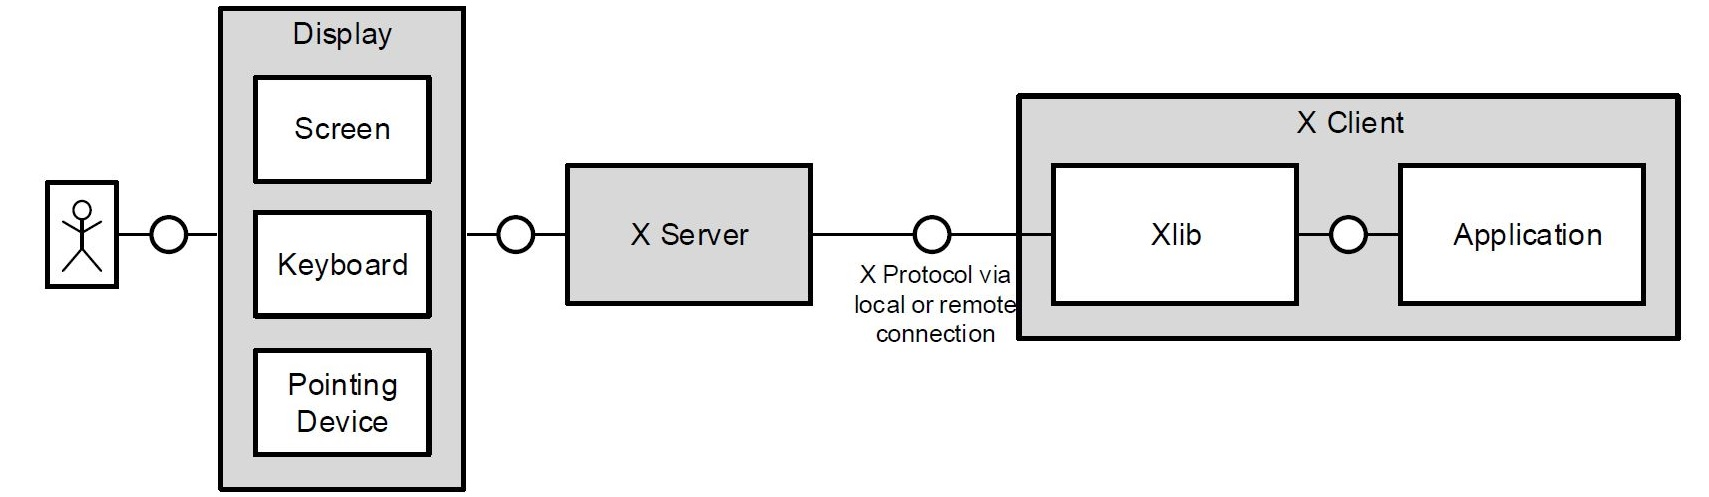
\includegraphics[width=1.0\linewidth]{04_X.JPG}
\begin{description}
  \item[Request] Client \textrightarrow~Server (Clientseitiger Buffer)
  \item[Replies] Client \textleftarrow~Server
  \item[Events] Client \textleftarrow~Server (Buff Server \& Client)
  \item[Errors] Client \textleftarrow~Server
  \item[X Ressource] Komplexe Ressourcen werden Serverseitig gehalten um Traffic zu reduzieren
  \item[Atom] ID eines Strings, verwendet um String parsing zu reduzieren (aka Konstante)
  \item[WM\textunderscore PROTOCOLS] Liste von Atome \& Protokollen
  \item[WM\textunderscore DELETE\textunderscore WINDOW] Window-Close-Event, Server \textrightarrow~Client
\end{description}



%UTF
\section{Encodings / Unicode}
\begin{description}
  \item[Coderaum] 17 × 2\textsuperscript{16} = 1'114'112 (128'237 in use)
  \item[Codepoint] Nummer eines Zeichens
  \item[Verbotene Codepoints] [D800] bis [DFFF]
  \item[Codeunit Längen] 8-bit, 16-bit, 32-bit
\end{description}

\subsubsection{UTF-8 (1-4 Codepoints, No Endian)}
\resizebox{1.0\linewidth}{!}{%
\begin{tabular}{lllll}
  Code-Point in & 1 & 2 & 3 & 4 \\
  \hline
  $[$0, 7F$]$ & 0xxx'xxxx & & & \\
  $[$80, 7FF$]$ & 110x'xxxx & 10xx'xxxx & & \\
  $[$800, FFFF$]$ & 1110'xxxx & 10xx'xxxx & 10xx'xxxx & \\
  $[$1'0000, 10'FFFF$]$ & 1111'0xxx & 10xx'xxxx & 10xx'xxxx & 10xx'xxxx \\
\end{tabular}%
}

\subsubsection{UTF-16 (1 oder 2 Codepoints, \underline{Endianness!})}
\resizebox{1.0\linewidth}{!}{%
\begin{tabular}{ll}
  Code-Point in & \\
   \hline
  $[$0, FFFF$]$ & Code-Unit = Code-Point\\
  $[$D800, DFFF$]$ & reserved (surrogate)\\
  $[$1'0000, 10'FFFF$]$ &   1101'10($[P_{20}$, $P_{16}]$-1)$[P_{15}$, $P_{10}]$1101'11$[P_{9}$, $P_{0}]$\\
  & in CU werden nur $[P_{19}$, $P_{0}]$ geschrieben
 \end{tabular}%
}
2 CU's resultierend $\rightarrow$ Surrogate-Pairs\\

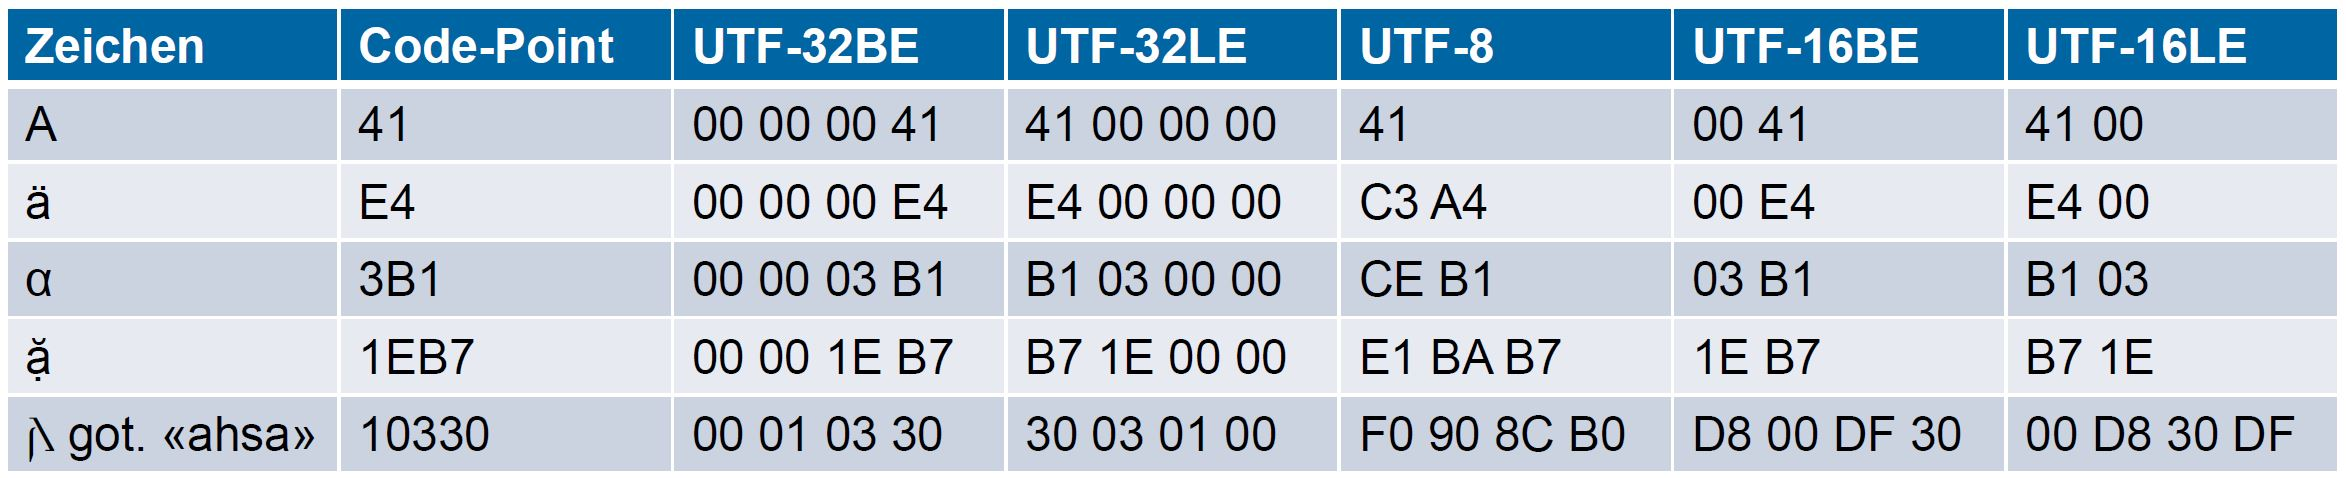
\includegraphics[width=1.0\linewidth]{05_Encodings.JPG}



%EXT
\section{Dateisysteme}
\begin{description}
  \item[Partition] Teilbereich des Datenträgers
  \item[Volume] Datenträger oder Partition
  \item[Sektor] kleinste logische Untereinheit von Volumen, Hardware definiert (traditionell 512 Bytes, modern 4KB), Header, Daten, Error-Correction-Codes
  \item[Format] Layout des Datenträgers (e.g. FAT, EXT4)
  \item[Block] mehrere subsequente Sektoren (1KB, 2KB, oder 4KB), gesamtes Volume wird in Blöcke aufgeteilt
  \item[Speicher] wird nur in Blöcken alloziert (leerraum!)
\end{description}

\subsection{Ext2}
\subsubsection{Inode}
\begin{description}
  \item[Index Node] Beschreibung einer Datei
  \item[Metadaten] der Datei, ausser Name \& Pfad (Grösse, Erzeugungs-, Zugriffzeit, ..., Owner, Flags, ...)
  \item[Fixe Grösse] je Volume: 2er Potenz, min. 128 Byte, max. 1 Block
  \item[Zeigt] auf Blöcke mit Filedaten
  \begin{description}
    \item[Blockliste] 60 Byte: 15 Blocknr. à 32Bit
    \item[0-12] für die ersten 12 Blöcke einer Datei
    \item[1] Blocknummer des indirekten Blocks
    \item[1] Blocknummer des doppelt-indirekten
    \item[1] Blocknummer des dreifach-indirekten
  \end{description}
  \item[Somit] 3-Dimensionen der Block-Allozierung (1KB Block \textrightarrow~\textgreater~16GB, 4KB Block \textrightarrow~\textgreater~4TB)
  \item[Fileholes] Blöcke voller 0en werden nicht alloziert
\end{description}

\subsubsection{Verzeichnisse}
\textbf{Entry}: Länge variabel 8 - 263 Bytes, aber immer Vielfaches von 4 Bytes\\
4 Bytes Inode, 2 Byte Length of Entry, 1 Byte Length of Name, 1 Byte File Type (1=Datei, 2=Verzeichnis, 7=Symbolischer Link), 0-255 Byte Name (Ascii)

\smallskip
\textbf{Links}
\begin{description}
  \item[Hardlink] Inode ist gleich
  \item[Symlink] Fake-Datei die auf andere Datei verweist
\end{description}

\smallskip
\textbf{Blockgruppe} Volume wird in Blockgruppen unterteilt\\
Gruppengrösse bis \textcolor{RoyalBlue4}{Faktor 8} der Anzahl Bytes pro Block\\
e.g. Blockgrösse 4 KB \textrightarrow~Gruppegrösse: $2^2KB x \textcolor{RoyalBlue4}{2^3} = 2^5K$ Blöcke pro Gruppe\\
Anzahl Blöcke pro Gruppe für alle Gruppen gleich\\
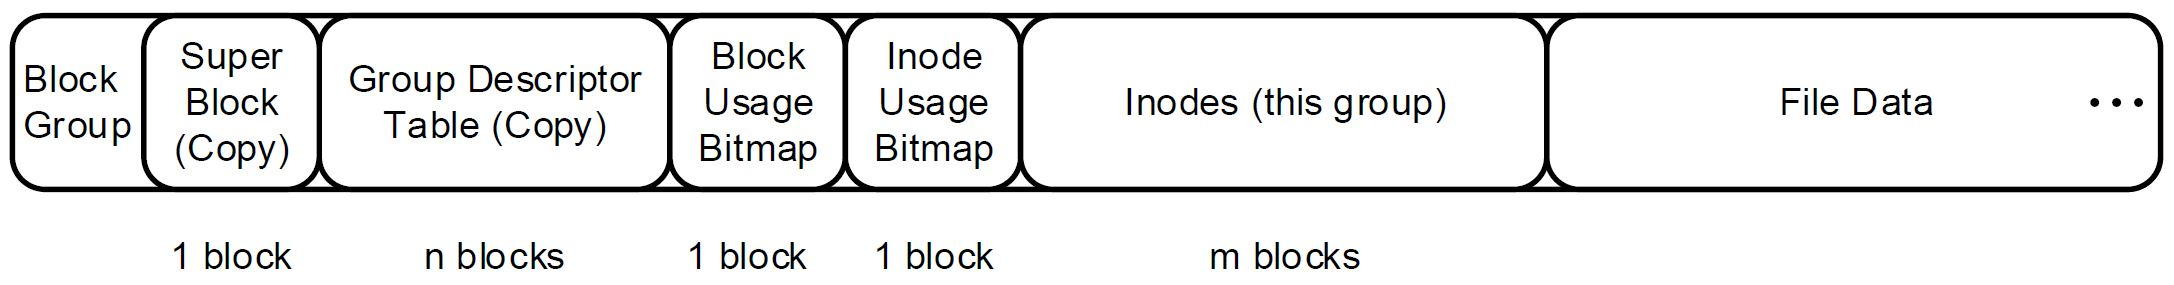
\includegraphics[width=1.0\linewidth]{06C_Block.JPG}

\smallskip
\textbf{Superblock} alle Meta-Daten über Volume (\textit{n}-Inodes, Bytes pro Block, ..., Zeitpunkte, Statusbytes, 1st Inode, Feature-Flags)\\
startet immer an Byte 1024 (Platz für Bootdaten)


\subsection{Ext4}
\begin{description}
  \item[Inodes] mit 256 Bytes statt 128, Gruppendeskriptor 64 statt 32, Blockgrösse bis 64KB
  \item[Extent Trees] Assoziation von Inodes via Baumstruktur (12Byte, max. 5 Ebenen)
\end{description}
\subsubsection{Journaling}
\begin{description}
  \item[Idee] Inkonsistenzen schneller überprüfen, da nicht alle Metadaten verifiziert werden müssen.
  \item[mode Journal] Daten werden komplett, ins Journal geschrieben, dann richtig, dann aus dem Journal entfernt.
  \item[mode Ordered] Nur Metadaten im Journal. Transaktion \textrightarrow~Dateiinhalte \textrightarrow~Commit. Dateien haben sicher richtigen Inhalt nach Commit, aber nicht optimale Performance.
  \item[mode Writeback] Nur Metadaten im Journal. Commit und Dateiinhalte schreiben in beliebiger Reihenfolge.
\end{description}



%ELF
\subsection{ELF}
Enthält Informationen für Linker und Loader. Enthält ELF Header,
Program Header Table (beschreibt Segmente die zur Laufzeit genutzt werden),
Section Header Table (beschreibt Sektionen für den Linker, meist nicht vorhanden
bei Objekt-Dateien) und Daten.

Segmente und Sektionen überlappen sich.

\begin{description}
  \item[.bss] Uninitialisierte Daten
  \item[.data] Initialisierte Date
  \item[.debug] Debug info
  \item[.rodata] Read-Only Daten
  \item[.text] Ausführbare Instruktionen
  \item[.symtab] Symbol-Tabelle. Spezifiziert Symbole mit Name (via
    Stringtabelle), z.B. Addresse, Grösse, Info
  \item[.strtab] String-Tabelle. Werden relativ zum Start der Tabelle
    referenziert, enthält z.B. Name von Symbolen.
\end{description}



%Libs
\subsection{Dynamische Libraries}

\textbf{GOT} \textit{global offset table} mit allen Adressen von sichtbaren Symbolen, Loader füllt die Addresse ein. Lazy binding.

\smallskip
\textbf{PLT} \textit{Procedure Linkage Table} zeigt auf eine Proxy-Funktion die lazy binding implementiert - sie sucht die Funktion und überschreibt GOT-Eintrag in Loader.

\smallskip
\begin{description}
  \item[linker name] libz.so (symlink auf soname). Vom Linker verwendet.
  \item[soname] libz.so.1 (symlink auf real name). Steht im Executable, wird vom
    Loader verwendet (da die Library mit der gleichen Major-Version
    ABI-kompatibel sein sollte)
  \item[real name] libz.so.1.2.11
\end{description}



%META
\section{author \& version}

Michael Stocker, \today

\end{multicols*}
\end{document}